\subsubsection{Logika gry}
\begin{par}
	Sama warstwa logiki gry podejmuje decyzje o relacjach pomiędzy obiektami w grze.
	Wszystkie elementy gry dziedziczą po klasie \textit{WorldObject}, która przechowuje podstawowe dane konieczne do wyświetlenia go w oknie takie jak położenie oraz wymiary.
	Kolejno możemy je podzielić na:
	\begin{itemize}
		\item Obiekt klasy \textit{Actor}. 
		Obiekt reprezentujący postać w grze. 
		Klasa ta posiada zmienną \textit{velocity}, oznaczającą wektor prędkości obiektu.  
		W każdym cyklu gry zostaje on dodany do położenia aktora.
		Na zmianę wektora wpływa klasa \textit{Controller} która w zależności od trybu gry przekazuje wciśnięcia klawiszy z klawiatury, lub akcje wygenerowane przez algorytm genetyczny.
		\item Obiekt klasy \textit{Terrain}. Z nich zbudowana jest mapa gry. Z punktu widzenia logiki nie wpływają one w żaden sposób na wynik, a jedynie kolidują z obiektem aktora. To z nich zbudowana jest mapa gry.
		\item Obiekty klasy \textit{Bonus}
		Są to obiekty wpływające na wynik gry. Kolizja Aktora z nimi powoduje zmianę wyniku gry. Klasa \textit{Bonus} jest klasą po której dziedziczą podklasy:
		\begin{itemize}
			\item BonusCoin - Obiekt reprezentujący punkty w grze. Aktorowi po kolizji z nimi zostaje dodana wartość punktowa przechowywana w obiekcie. Z punktu widzenia algorytmu zwiększają one ostateczną wartość funkcji przystosowania, która zależy od ilości punktów zebranych na mapie.
			\item BonusWin - Kolizja aktora z obiektem tego typu kończy przejście chromosomu bądź gracza i zapisuje w stanie gry wynik końcowy \textit{RESULT\_WON}. W praktyce oznacza on zakończenie gry z pozytywnym skutkiem, który jest brany pod uwagę podczas wyliczenia funkcji przystosowania.
			\item BonusLose - Obiekt kończący grę ze skutkiem negatywnym. Ma on reprezentować wszelkiego rodzaju pułapki w grze, które natychmiastowo kończą przejście chromosomu. W stanie gry zostaje wówczas zapisany wynik końcowy \textit{RESULT\_LOST}.
		\end{itemize}
	\end{itemize}
	\definecolor{orange}{rgb}{1,0.5,0}
	\definecolor{gray}{rgb}{0.5,0.5,0.5}
	Na rysunku \ref{fig:objects} widać obiekty świata gry: 
	\textcolor{blue}{\textit{Actor}}, 
	\textcolor{orange}{\textit{BonusCoin}},
	\textcolor{red}{\textit{BonusLose}},
	\textcolor{green}{\textit{BonusWin}},
	\textcolor{black}{\textit{Terrain}}.

	\begin{figure}[!h]
		\centering
		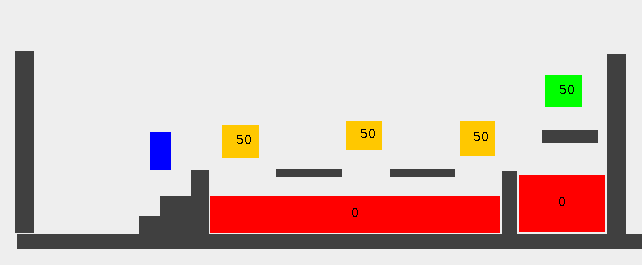
\includegraphics[width=4in]{obrazki/objects.png}
		\caption{Poszczególne elementy mapy.}
		\label{fig:objects}
	\end{figure}
\end{par}

\begin{par}
	Podstawową logiką gry i detekcją kolizji pomiędzy obiektami zarządza obiekt klasy \textit{LogicMario}. Użytym w pracy schematem logiki jest schemat gry ``Super Mario Brothers''. 
	Zakłada ona ruch w 2 kierunkach, skok oraz działanie grawitacji na obiekt aktora.
	Ponieważ klasa \textit{LogicMario} dziedziczy po klasie \textit{Logic} możliwe jest napisanie własnej logiki i podmiana tej obowiązującej w systemie.
	Ponieważ działanie algorytmu nie jest związane z fizyką ani zasadami obowiązującymi w grze, system może działać dla wielu różnych typów gier platformowych i zręcznościowych, pod warunkiem że dają się one opisać za pomocą wyżej zdefiniowanych klas i cech(\textit{WorldObject}, rezultaty zakończenia gry, rodzaje możliwych akcji do wykonania).
\end{par}

